%!TEX root = ../../thesis.tex

\section{Simulation and results}
\label{sec:chi2_results}

%!TEX root = ../thesis.tex

\begin{table*}
      \centering
      \begin{threeparttable}
          \caption{Input and recovered parameters on simulations and an observation when applying a single (\(\rm C^1\)) and binary (\(\rm C^2\)) models. The \logg{} and metallicity were fixed at \(\logg{}_1 = 4.50\), \(\logg{}_2=5.0\) and \feh{}=0.0 equally for both components. Gaussian noise was added to both simulations with a \snr{} of 150. Here \(m\) and \(n\) are the number of data points and parameters used in each model.}

          \begin{tabular}{c | *3c | *3c | *3c}
              \toprule
              & \multicolumn{3}{c|}{Simulation 1} & \multicolumn{3}{c|}{Simulation 2} & \multicolumn{3}{c}{Observed {HD 211847}} \\
              \midrule
          & Input & \multicolumn{2}{c|}{Recovered} & Input & \multicolumn{2}{c|}{Recovered} & Expected & \multicolumn{2}{c}{Recovered} \\
          & & \(C^1\) & \(C^2\) & & \(C^1\) & \(C^2\) & & \(C^1\)  & \(C^2\) \\
          \midrule
          \(\teffsub{1}\) & 5\,800 & 5\,800 & 5\,800 & 5\,700 & 5\,800 & 5\,700 & \(5\,715 \pm 24\) & 5\,900 & 5\,800\\
          \(\teffsub{2}\) & 4\,000 & -- & 3\,800 & 3\,200 & -- & 3\,100 & \(\sim\)3\,200 & -- & >3\,800\tnote{a}\\
          \({rv}_1\) & 0 & 0.1 & 0 & 6.6 & 6.6 & 6.6 & \(6.6 \pm 0.3\) & 7& 7.6 \\
          \({rv}_2\) &  10 & -- & 9.8 & 0.5 & -- &  -1& \(0.5 \pm 2\) & -- &-12.6\\
          \midrule
          \(R_1/R_2\)& 2.57 & -- & 2.71& 3.16 & - & 3.27 & 3.16 & -- & <2.71\tnote{a}\\
          \(\rm F_2/F_1\)& 0.084 & -- & 0.066 & 0.030 & -- & 0.026 & 0.030 & -- & >0.066\tnote{a}\\
          \(m\) & - & 3\,072 & 3\,072 & -- & 3\,072 & 3\,072 & -- & 2\,612 & 2\,612\\
          \(n\) & - & 2 & 4 & -- & 2 & 4 & -- & 2 & 4\\
          \textchisquared& -- & 4\,978 & 3\,792 & -- & 3\,746 & 3\,630  & -- & 37\,688 & 33\,860\\
          \(\chisquared_{red}\) & -- & 1.62 & 1.24 & -- & 1.22 & 1.18 & -- & 21.3 & 19.2\\
          {BIC} & -- & -20\,145 & -22\,315 & -- & -21\,477 & -21\,377& -- & 18\,281 & 14\,468\\
          \bottomrule
        \end{tabular}\label{tab:example_params}
        \begin{tablenotes}
            \item [a] {At the arbitrary upper limit for companion temperature grid (3\,800\K{}).}
        \end{tablenotes}
    \end{threeparttable}
\end{table*}


\begin{figure*}
    \centering
    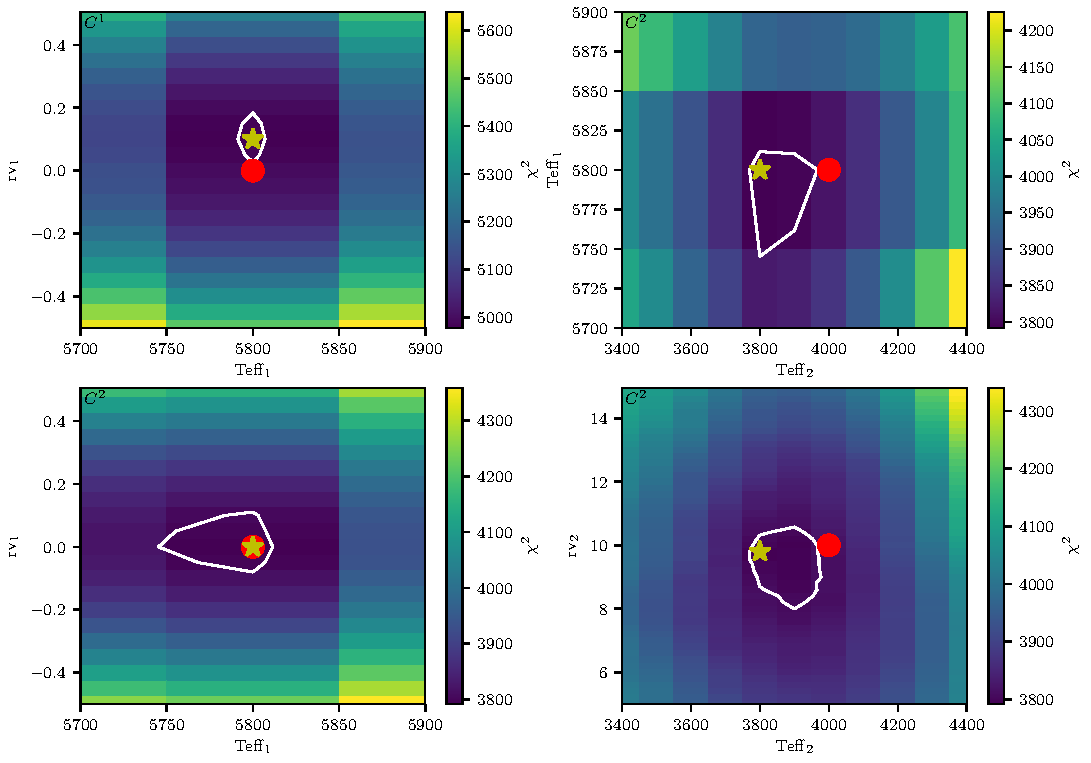
\includegraphics[width=0.7\linewidth]{figures/companion_recovery/Mdwarf_pcolors}
    \caption[\textchisquared{} contour for companion recovery of a simulated Sun - M-dwarf binary.]{\textchisquared{} results for companion recovery of a simulated binary observation of a Sun-like star (\(\teffsub{1}=5800\)\K{}) with an M-dwarf companion (\(\teffsub{2}=4000\)\K{}).
        The top right plot shows the application of a single component model (\(C^1\)) while the other three are using a binary model (\(C^2\)).
        Both left hand panels show the distribution of host temperature and host {RV}.
        The top right panel shows the distribution for host and companion temperature, and the bottom right the companion temperature and radial velocity.
        The red circle and yellow star indicate the location of the simulation input and recovered parameters respectively.
        The white line shows a 3-\(\sigma\) confidence level about the minimum \textchisquared{} solution grid point.
        Each box is centred on the parameter values and shows the grid resolution.}
    \label{fig:Mdwarf_contours}
\end{figure*}

\begin{figure*}
    \centering
    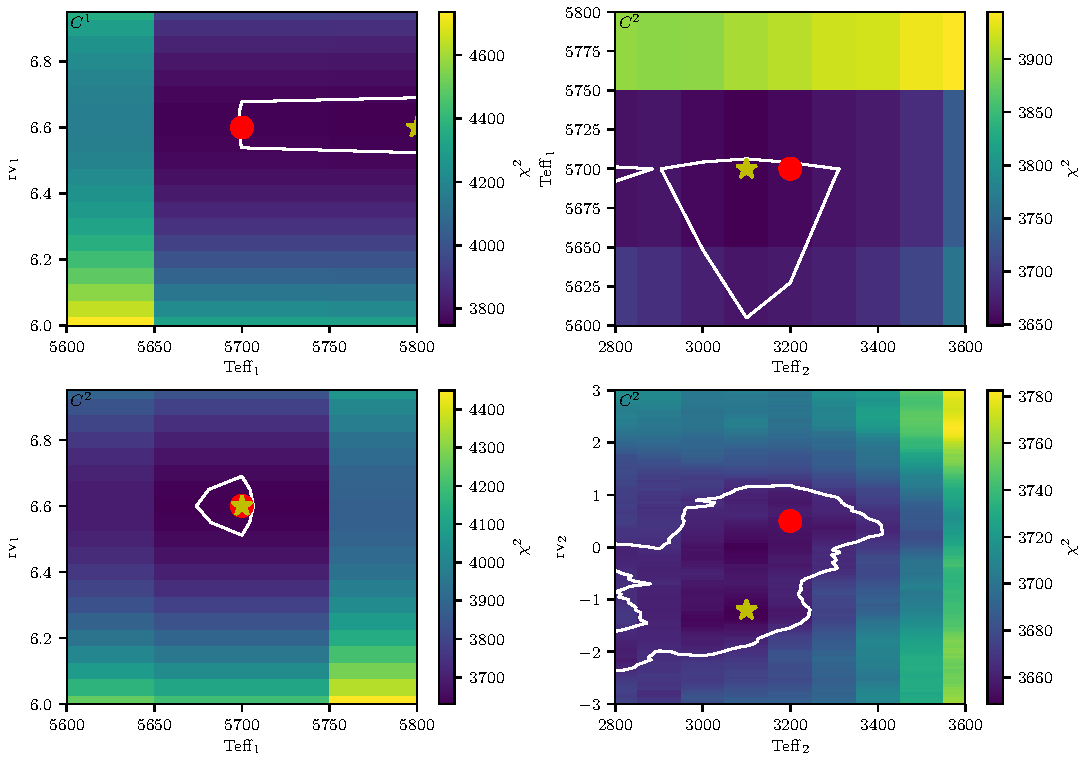
\includegraphics[width=0.7\linewidth]{figures/companion_recovery/HD211847_example_pcolors}
    \caption[\textchisquared{} contour for companion recovery of a simulated observation of {HD 211847}.]{ \textchisquared{} results for companion recovery of a simulated binary observation similar to {HD 211847}, \(\teffsub{1} = 5800\)\K{}, \(\teffsub{2} = 3200\)\K{}, similar to \cref{fig:Mdwarf_contours}.}
    \label{fig:HD211847_simulated_contours}
\end{figure*}

In this section some results from applying the models for companion recovery model to simulated observations and to the observed target with the best estimated contrast are presented.

\subsection{Simulated binaries}
\label{subsec:simulated_binaries}
To test the companion recovery method simulations of binary observations using {PHOENIX-ACES} spectra were performed.
These are performed in the wavelength range between 2112--2152\nm{}, covering the first three detectors of CRIRES only, due to spectral mismatch observed later in the observed spectra.
White noise was added to the simulated spectra a standard deviation \(\sigma = 1/{\snr{}}\), for a given signal-to-noise (\snr{}) level.
The \textchisquared{} grid-search recovery technique detailed above is applied and the resulting parameters compared to the inputs.

The results of two example binary simulations are displayed in \cref{fig:Mdwarf_contours,fig:HD211847_simulated_contours}, both simulated with a \snr{} of 150.
In each figure the input and recovered parameters for the binary components are indicated by the red circles and yellow stars respectively, and are given in \cref{tab:example_params}.
The 3-\(\sigma\) contour is shown with a white line on the plots to indicate the shape of the confidence level only.
The 1-\(\sigma\) contours are not shown here as they are much smaller than the temperature grid step and are difficult to visualize at this scale, often being smaller than the marker shown at the location of the minimum \textchisquared{}.
Each coloured rectangle is centred on a grid point, with its colour indicating the \textchisquared{} value, and its shape indicating the resolution of the parameter grid space searched.

\subsubsection*{M-dwarf companion}
The first simulation is for a Sun-like star with a M-dwarf companion with temperatures \(\teffsub{1} = 5800\)\K{}, \(\teffsub{2} = 4000\)\K{}.
The results are shown in \cref{fig:Mdwarf_contours}.
The top-left panel shows the recovered host parameters when only the single model is fitted to the spectra of the simulated binary.
The top-right and both bottom panels show different parameter slices recovered when fitting with the binary model.
Both left-hand panels display the parameters for the host, \(\teffsub{1}\) and \Rvone{}, to easily compare between the two models.
With both models the host temperature \(\teffsub{1}\) is exactly recovered.
The recovered host {RV}, \Rvone{}, is 0.1\kmps{} (two grid spaces) different from the input value in the single component model and is correctly recovered with the binary model.

For the companion the minimum \textchisquared{} location for the companion temperature is 200\K{} below the simulated value, and the {RV} of the companion recovered is 0.2\kmps{} below the input value.
The input values for the companion are just outside of the 3-\(\sigma\) contours shown.
The flux ratio for the input is 0.08 while the flux ratio recovered is 0.066.
This begins to show the difficulty of recovering the companion.

\subsubsection*{{HD~211847} simulation}
A second simulation is performed with parameters to mimic the observation of the target with highest flux ratio, {HD 211847}, and is shown in \cref{fig:HD211847_simulated_contours}.
In this simulation the single component model recovers a host with the correct {RV} but a temperature 100\K{} higher than the input value (one grid step).
Again, adding the companion with the binary model recovers the correct host temperature.
The companion temperature recovered is 100\K{} lower than the input temperature and the {RV} is different by 2\kmps{} which is around one third the {\fwhm}.

In this case with a companion {RV} offset, \Rvtwo{}, near 0\kmps{} the host and companion lines are blended.
The same spectral lines from both components are trying to match the same features of the spectra, making it more difficult to recover the companion parameters.
In the bottom right panel there appears to be multiple minima for different \Rvtwo{} and \(\teffsub{2}\) combinations, with a complex 3-\(\sigma\) confidence contour.
This is assumed to be partially due to the small \Rvtwo{}.

From the result summary in \cref{tab:example_params}, both simulations have a \textchisquaredreduced{} for the binary model closer to 1 than the single model.
This is not surprising as the binary model contains extra parameters.
As mentioned above, care is needed, as the extra components from the binary may just happen to fit components of the noise when a binary is not present, or at a extreme low contrast ratio as in this case.
To further analyse the significance between the two models the ``Bayesian Information Criterion'' ({BIC})~\citep{schwarz_estimating_1978} is used:
\begin{equation}
{BIC} = n\ln{(m)} - 2\ln{(\hat{L})}.
\end{equation}
Here \(n\) and \(m\) are the number of parameters and number of data points respectively and \(\hat{L}\) is the maximum of the Gaussian likely-hood function, 
\begin{equation}
\hat{L} = {\left(\frac{1}{\sigma \sqrt{2\pi}}\right)}^{m} \exp{\left(-\frac{\chisquared}{2}\right)},
\end{equation}
written in terms of \textchisquared{} and a fixed \(\sigma\) for all data points.
The maximum likely-hood of a Gaussian distribution is equivalent to minimizing the \textchisquared{}.
In both simulations the change in {BIC} between models, \(\Delta {BIC} >10\), so the preference of the binary model, with the lower {BIC} value, over the single component model is considered \emph{significant}.

\subsection{HD211847 observation}
\label{subsec:results-hd211847}
{HD 211847} is the best candidate of the current targets for companion detection with the \textchisquared{} binary model as it has a 155\Mjup{} low-mass star companion~\citet{moutou_eccentricity_2017}.
Even though it has been determined not a {BD} in the literature it has the highest estimated flux ratio out of the current sample, of 0.03 based on the~\citet{baraffe_new_2015} evolution models and the known companion mass (see \cref{tab:estimated_flux_ratios}).
\citet{moutou_eccentricity_2017} used Angular Differential Imaging {ADI} with {SPHERE@VLT} to observe an angular separation of the two bodies of 219.6\mas{} corresponding to a projected separation of 11.3\AU{}. For comparison the {CRIRES} slit with on the sky is 400\mas.
However, it was not determined if the orientation of the orbit was considered during the observation, to align the slit along the orbit.
The result of applying \textchisquared{} fitting to the second observation of {HD 211847} is given in \cref{tab:example_params} and visualized in \cref{fig:HD211847_result_contours}.

For the fitting of this target the metallicity of both components was fixed to 0.0 and the \Logg{} for the host was fixed at 4.5.
The \Logg{} for the companion is also fixed to 5.0, based on the~\citet{baraffe_new_2015} evolutionary models for the given companion mass and system age.
The orbital solution of the target was used to define the initial {RV} search space of both components, however the first range for the companion {RV} was too narrow and was extended until the companion was recovered with a value inside the {RV} bounds.

Again the top left panel of \cref{fig:HD211847_result_contours} shows the recovery with a single component model with the other three displaying parameter slices of the binary model.
Here the red circle marks the location of the expected values from the literature while the yellow star indicate the location of the minimum \textchisquared{} recovered parameters.
There error bar on the host temperature also comes from the literature, while the error on estimated {RV} values, shown in \cref{fig:HD211847_result_contours}, is calculated by applying the general error propagation formula~\citep{ku_notes_1966} to the {RV} equation (\cref{eqn:rv2_equation}) and using the errors on the published orbital parameters.
For a function, \(f\), with errors on the inputs \(\delta x\), \(\delta y\) etc., it follows:
\begin{align}
f &= f(x, y, z, \ldots)\\
\delta f &= \sqrt{{\left( \frac{\partial f}{\partial x} \delta x\right)}^2 + {\left(\frac{\partial f}{\partial y} \delta y\right)}^2 + {\left(\frac{\partial f}{\partial z} \delta z\right)}^2 + \ldots}.
\end{align}

The fitted single component model finds a temperature of 5900\K{} for the host with a \Rvone{} of 7\kmps{}.
This is 200\K{} and 0.4\kmps{} different above the expected parameters.
The binary model finds a host temperature of 5800\K{}, which is the second closest model to the literature value, <100\K{} different.
The host {RV} value recovered with the binary model is 7.6\kmps{}, which is 1\kmps{} higher than expected, but again these {RV} differences are smaller than the {\fwhm} of the lines.
For the single component model there is a barely noticeable evidence of a secondary minima near this 7.6\kmps{} {RV} value which is recovered by the binary model.
The 3-\(\sigma\) contour in these plots is small due to the large gradient of the \textchisquared{}, it is just visible on the right hand side of the star in the bottom left panel, and hidden behind the markers in the other panels.

For the companion in the binary model, on the right side of \cref{fig:HD211847_result_contours} shows a problem.
The minimum \textchisquared{} for the companion temperature is at the upper limit of the grid shown.
If the grid extend is extended the companion temperature towards higher temperatures the best fit location continues to increase in the recovered temperature, continually hitting the upper limit until it is close to the host temperature, more than 2000\K{} above the expected companion temperature.
When the companion temperature becomes this high it also affects the recovered parameters for the host star to offset the features of the brighter companion.
Also the companion {RV} is >12\kmps{} different than the expected value, around two line \fwhm{}s away.
Obviously this is not correct and the actual companion is not being detected.

The \textchisquaredreduced{} values for the single and binary models are 21 and 19 respectively, far from the value of 1, indicating that both models are a poor fit to the observations.
The \(\Delta {BIC} = 3812 >10\) indicating that the binary model is preferred, i.e.\ the difference is \textit{significant}.

The spectrum of the best fit solution binary model is shown against the observed spectra in \cref{fig:visualinspection-hd2118471}.
It is observed that there is a large spectral mismatch between the synthetic models and the observed spectra.
Extra wavelength masking was applied to many of the largest mismatched synthetic lines to remove their influence on the \textchisquared{}.
The grey areas mark regions which have been masked out, either from the centres of deep telluric lines (the thin masks matching spectral gaps), or the more prominent mismatched lines in the synthetic spectrum excluded from the \textchisquared{} analysis.
One clear example of a mismatched line is a synthetic line at 2132.5\nm{} that is clearly not observed in detector \#2 (top right).
Even with the majority of the mismatched lines removed the detection of the companion was still unsuccessful.
The shown results for the observed spectra include the wavelength masking.

For detectors \#1 and \#2 it appears that the synthetic spectra contain many more deeper lines than observed.
For detector \#3 the red half of the detector was masked out as there appears to be an {RV} offset between the observed lines and synthetic spectra.
With 3--4 lines that appear to be consistently offset from the observation it could be a wavelength calibration issue, although the telluric lines appear to be sufficiently corrected in this region, attesting for the quality of the wavelength calibration, and making it incompatible with the offset.

For detector \#4 the observed lines do not agree at all with the models.
With many observed lines not in the model and only one line with some agreement in wavelength, detector \#4 is masked out completely and not used in the \textchisquared{} fit of the simulation or observed spectral fitting..
Individual inspection of the \textchisquared{} results for each detector also revealed that there was a large discrepancy between the \nth{4} detector and the other three, with a different {RV} value for the host star and a \textchisquared{} values an order of magnitude higher.
The edge of a deep Hydrogen line (Brackett-\(\gamma\)) off the edge of the detector \#4 is also clearly seen in the continuum of the model >2162\nm{}, and possibly part of the reason for the poor fitting.

The same method was applied the remaining targets, all with similar results for the companion, having companion spectra well above the expected values.
In brief, it is conclude that the companion spectra cannot be correctly detected in the observation presented here using this method.

\begin{figure*}
    \centering
    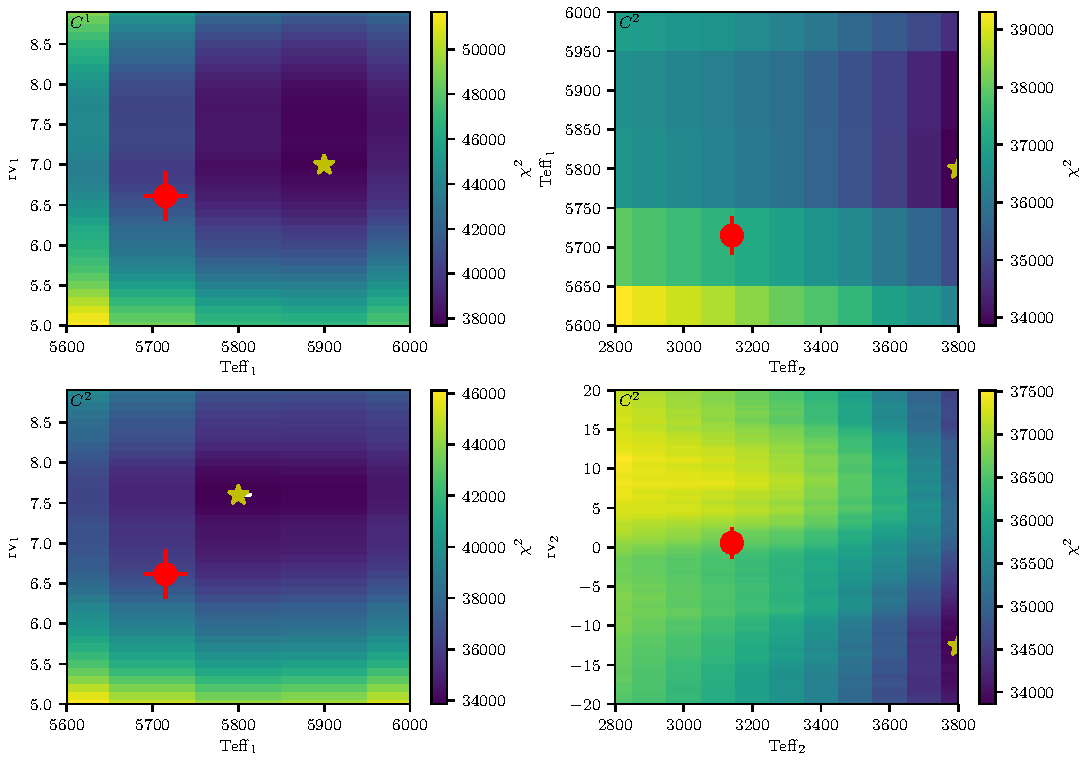
\includegraphics[width=0.7\linewidth]{figures/companion_recovery/HD211847_result_pcolors}
    \caption[\textchisquared{} contour for an observation {HD 211847}.]{\textchisquared{} result grid for the second observation of {HD 211847}, similar to \cref{fig:Mdwarf_contours,fig:HD211847_simulated_contours}.
        The white line shows a 3-\(\sigma\) confidence level about the minimum \textchisquared{} solution grid point, not always visible here due to the large \textchisquared{} values.
        The error bar on \(\teffsub{1}\) is from the literature while the error bars on \Rvone{} and \Rvtwo{} are calculated by propagating the orbital parameter uncertainties though the radial velocity equation (\cref{eqn:rv_equation_intro}).}
    \label{fig:HD211847_result_contours}
\end{figure*}

\begin{figure*}
    \centering
    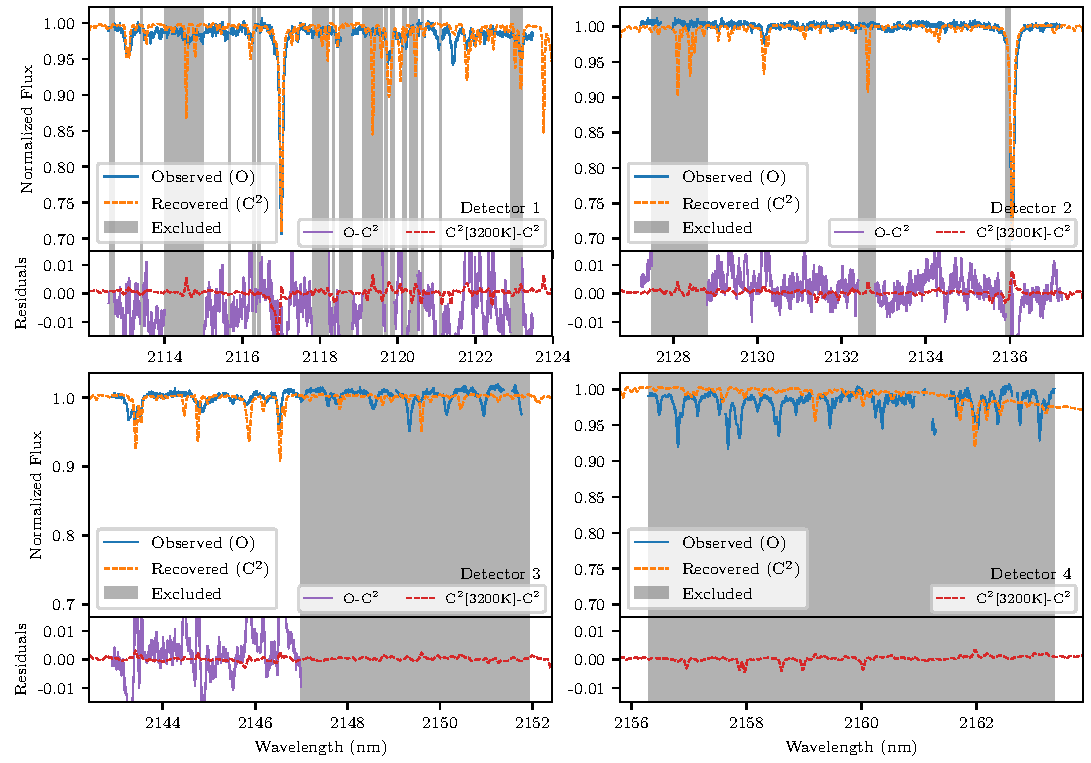
\includegraphics[width=0.7\linewidth]{figures/companion_recovery/visualize_result_residuals}
    \caption[Comparison between observation of {HD 211847} and the best fit synthetic binary model.]{Comparison between the observed {HD 211847} spectrum (blue) and the best fit synthetic binary model (orange dashed) for each detector.
        The bottom section of each panel shows the residuals between the parts of the observation used in the \textchisquared{} fit and recovered binary model (\(\rm O-C^2\)) in purple.
        The red dashed line shows the difference between the recovered binary model and the binary model with the exact same parameters except for the estimated companion temperature of 3200\K{} (\(\rm C^2[3200\K{}]- C^2\)).
        The grey shading indicated the wavelength regions where masking has been applied.
        The thinner masked regions that match with cuts in the observed spectra are where the centres of deep (>5\%) telluric lines that have been masked out are.}
    \label{fig:visualinspection-hd2118471}
    %\label{fig:visualizeresultresiduals}
\end{figure*}
